\section{System Architecture}
\label{sec:architecture}

WuYa employs a two-phase routing architecture centered around a Router agent that orchestrates specialized \subagents{} for academic paper evaluation. This section details the architectural components, including the two-phase routing mechanism, \subagent{} designs, and the hybrid knowledge strategy.

\subsection{Overall Architecture}

Figure~\ref{fig:architecture} presents the overall system architecture. The Router serves as the central orchestrator, responsible for:

\begin{enumerate}
    \item \textbf{Paper parsing}: Extracting content, metadata, and key features from input papers.
    \item \textbf{Intent recognition}: Determining whether the request is for submission recommendation or journal review.
    \item \textbf{Two-phase routing}: Dispatching tasks to appropriate \subagents{} based on the evaluation workflow.
    \item \textbf{Result aggregation}: Combining outputs from multiple \subagents{} into coherent recommendations or reviews.
\end{enumerate}

\begin{figure}[t]
    \centering
    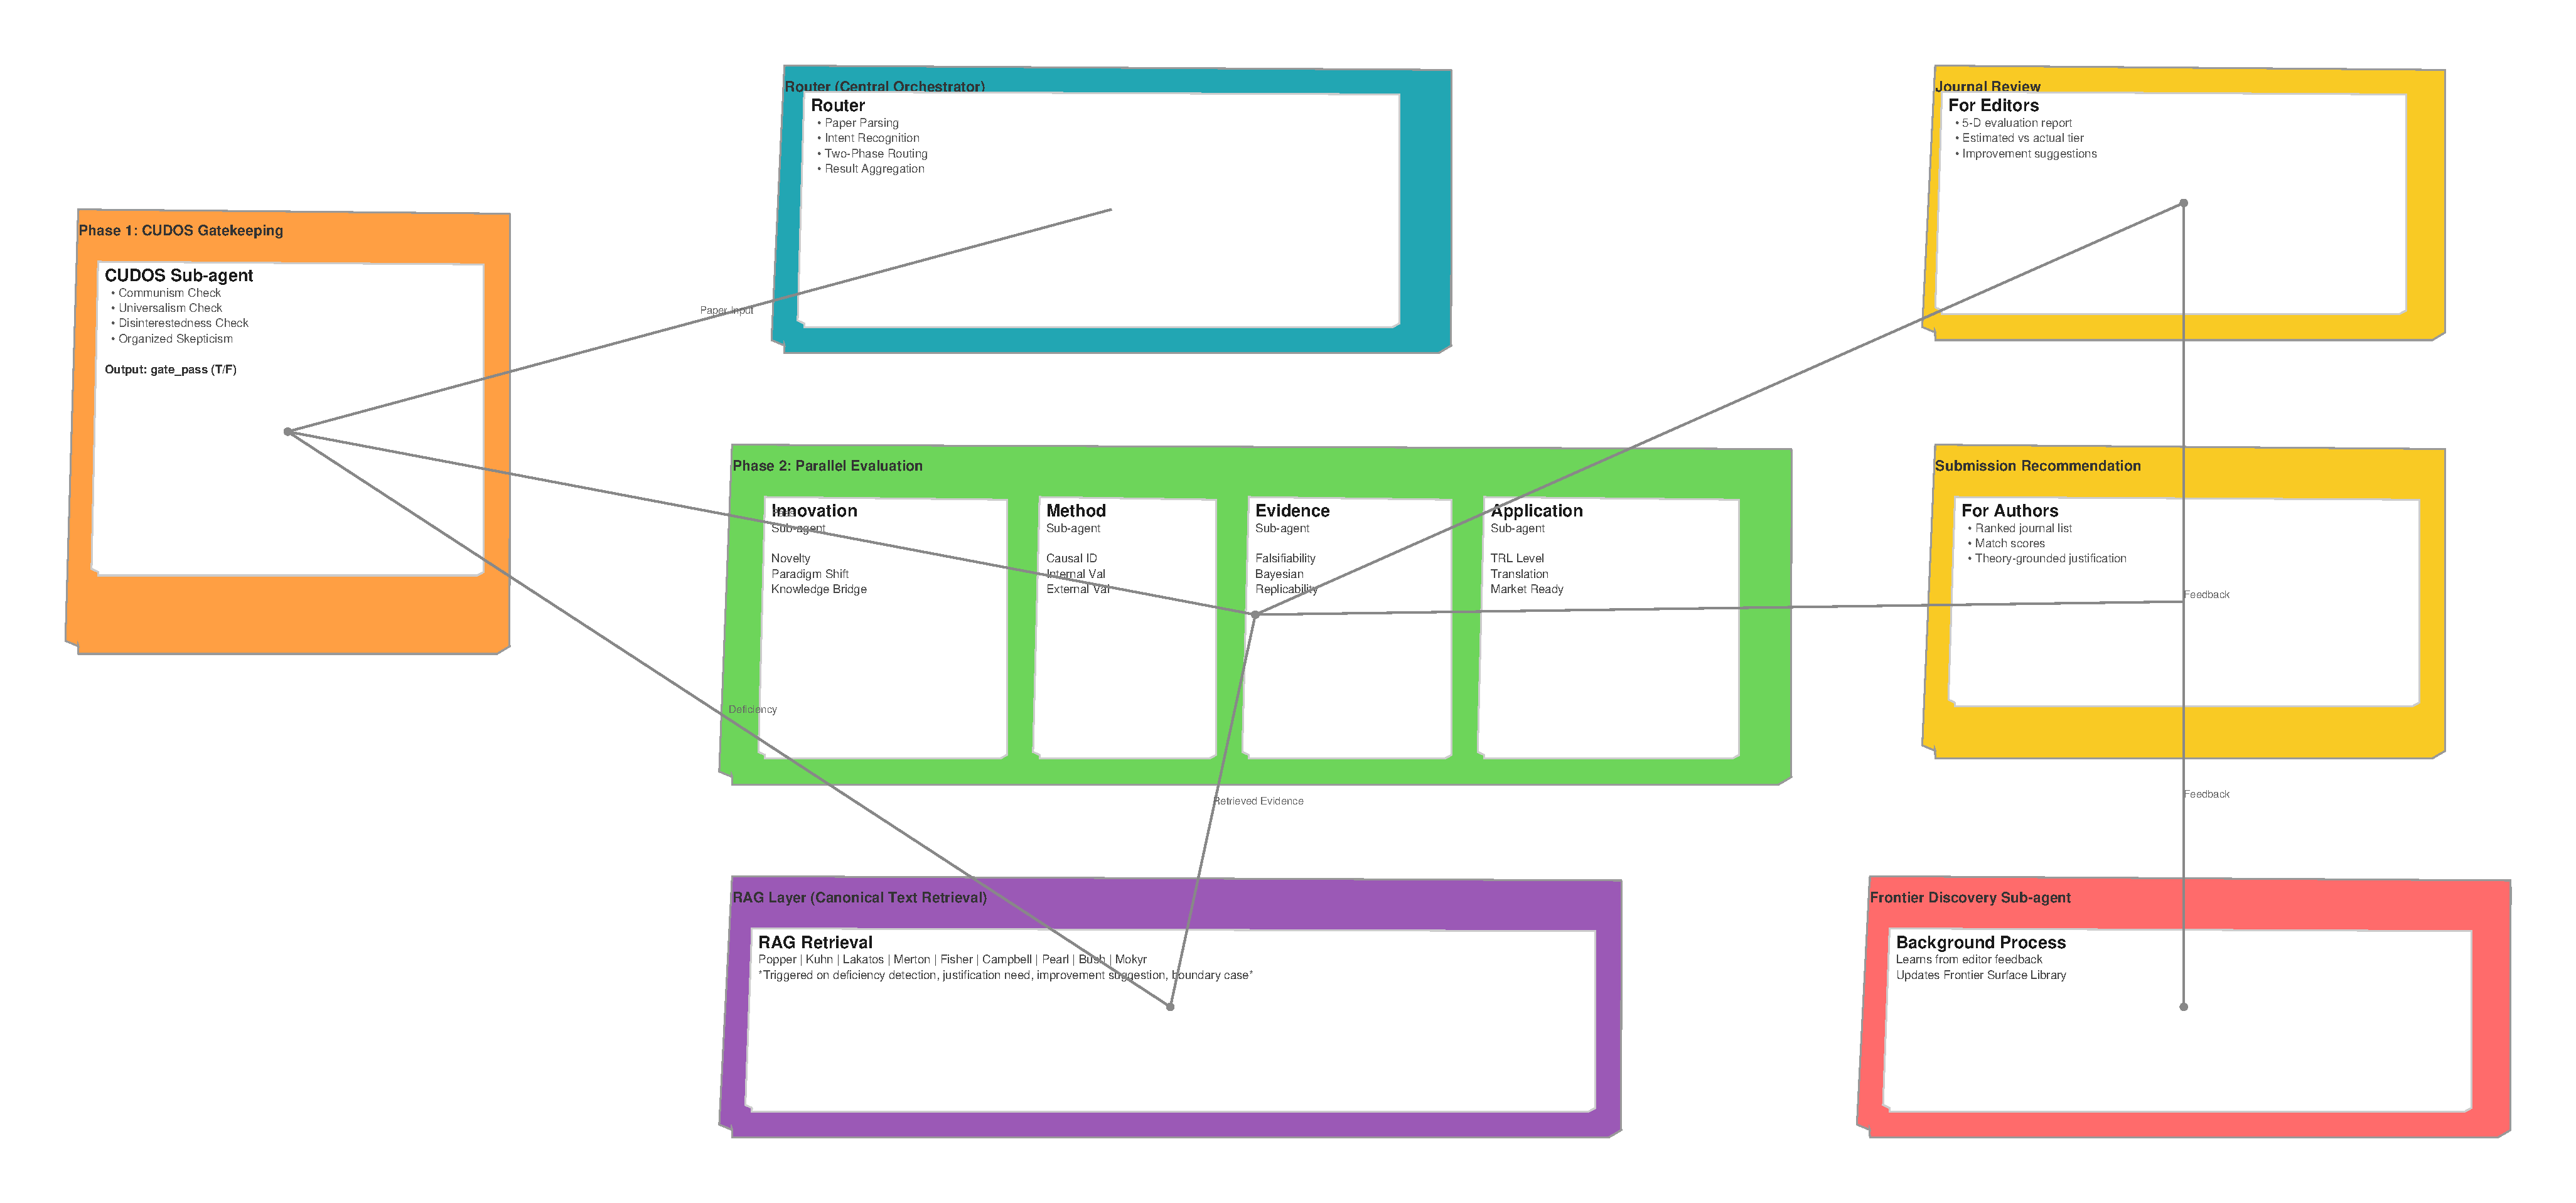
\includegraphics[width=\textwidth]{figures/architecture.pdf}
    \caption{WuYa System Architecture: Two-Phase Routing with Parallel Evaluation}
    \label{fig:architecture}
\end{figure}

The system supports two user scenarios:
\begin{itemize}
    \item \textbf{Submission Recommendation}: For authors seeking to identify appropriate target journals for their papers.
    \item \textbf{Journal Review}: For editors seeking AI-assisted evaluation of submitted manuscripts.
\end{itemize}

\subsection{Two-Phase Routing}

The two-phase routing design reflects a fundamental principle: norms (\cudos{}) must be assessed before substantive quality. This separation ensures that the Router's scheduling responsibilities do not interfere with the CUDOS \subagent{}'s evaluative judgment.

\textbf{Phase 1: CUDOS Gatekeeping.} The CUDOS \subagent{} evaluates the paper against Merton's four normative principles:
\begin{itemize}
    \item Does the paper share knowledge openly (Communism)?
    \item Are evaluation criteria objective (Universalism)?
    \item Does the research aim at truth rather than personal gain (Disinterestedness)?
    \item Does the work invite critical scrutiny (Organized Skepticism)?
\end{itemize}
If the CUDOS \subagent{} returns \texttt{gate\_pass: false}, the paper is rejected with a detailed explanation of normative concerns, and Phase 2 is not executed. This implements the ``gatekeeping'' semantics where violations of scientific norms trigger immediate rejection.

\textbf{Phase 2: Parallel Expert Evaluation.} Upon passing CUDOS, four expert \subagents{} execute in parallel:
\begin{itemize}
    \item \textbf{Innovation Sub-agent}: Evaluates novelty, paradigm shift potential, and knowledge bridging.
    \item \textbf{Method Sub-agent}: Assesses causal identification, internal/external validity, and statistical rigor.
    \item \textbf{Evidence Sub-agent}: Evaluates falsifiability, evidence strength, replicability, and research programme alignment.
    \item \textbf{Application Sub-agent}: Assesses TRL level, translation path, and market readiness.
\end{itemize}

Each \subagent{} produces structured output including sub-dimension scores (1-5 scale) and narrative explanations. The Router aggregates these into a unified \textbf{five-dimensional score vector}.

\subsection{Retrieval-Evaluation Coupling}

A key innovation in WuYa is the tight coupling between evaluation and retrieval. Unlike systems where \rag{} serves as a passive knowledge source, WuYa's \rag{} is triggered by evaluation conditions:

\begin{algorithm}[t]
\caption{Retrieval-Evaluation Coupling}
\label{alg:rag-trigger}
\begin{algorithmic}
\STATE Initialize score\_vector
\FOR{each evaluation sub-agent}
    \STATE Generate initial evaluation based on internalized principles
    \IF{evaluation reveals deficiency OR needs justification}
        \STATE Identify relevant theory and concept
        \STATE Retrieve canonical passages via RAG
        \STATE Incorporate retrieved evidence into evaluation
    \ENDIF
\ENDFOR
\STATE Return enriched score\_vector with citations
\end{algorithmic}
\end{algorithm}

The triggering conditions include:

\begin{enumerate}
    \item \textbf{Deficiency detection}: When an evaluation finds a weakness in the paper (e.g., ``the hypothesis lacks falsifiability'').
    \item \textbf{Justification need}: When a judgment requires authoritative support (e.g., ``this is problematic because...'').
    \item \textbf{Improvement suggestion}: When actionable guidance is needed (e.g., ``to improve, consider...'').
    \item \textbf{Boundary case}: When the paper falls in a gray area of the evaluation criteria.
\end{enumerate}

This coupling transforms evaluation from static judgment to dynamic reasoning with principled justification.

\subsection{Hybrid Knowledge Strategy}

WuYa implements a dual-layer knowledge architecture:

\begin{figure}[t]
    \centering
    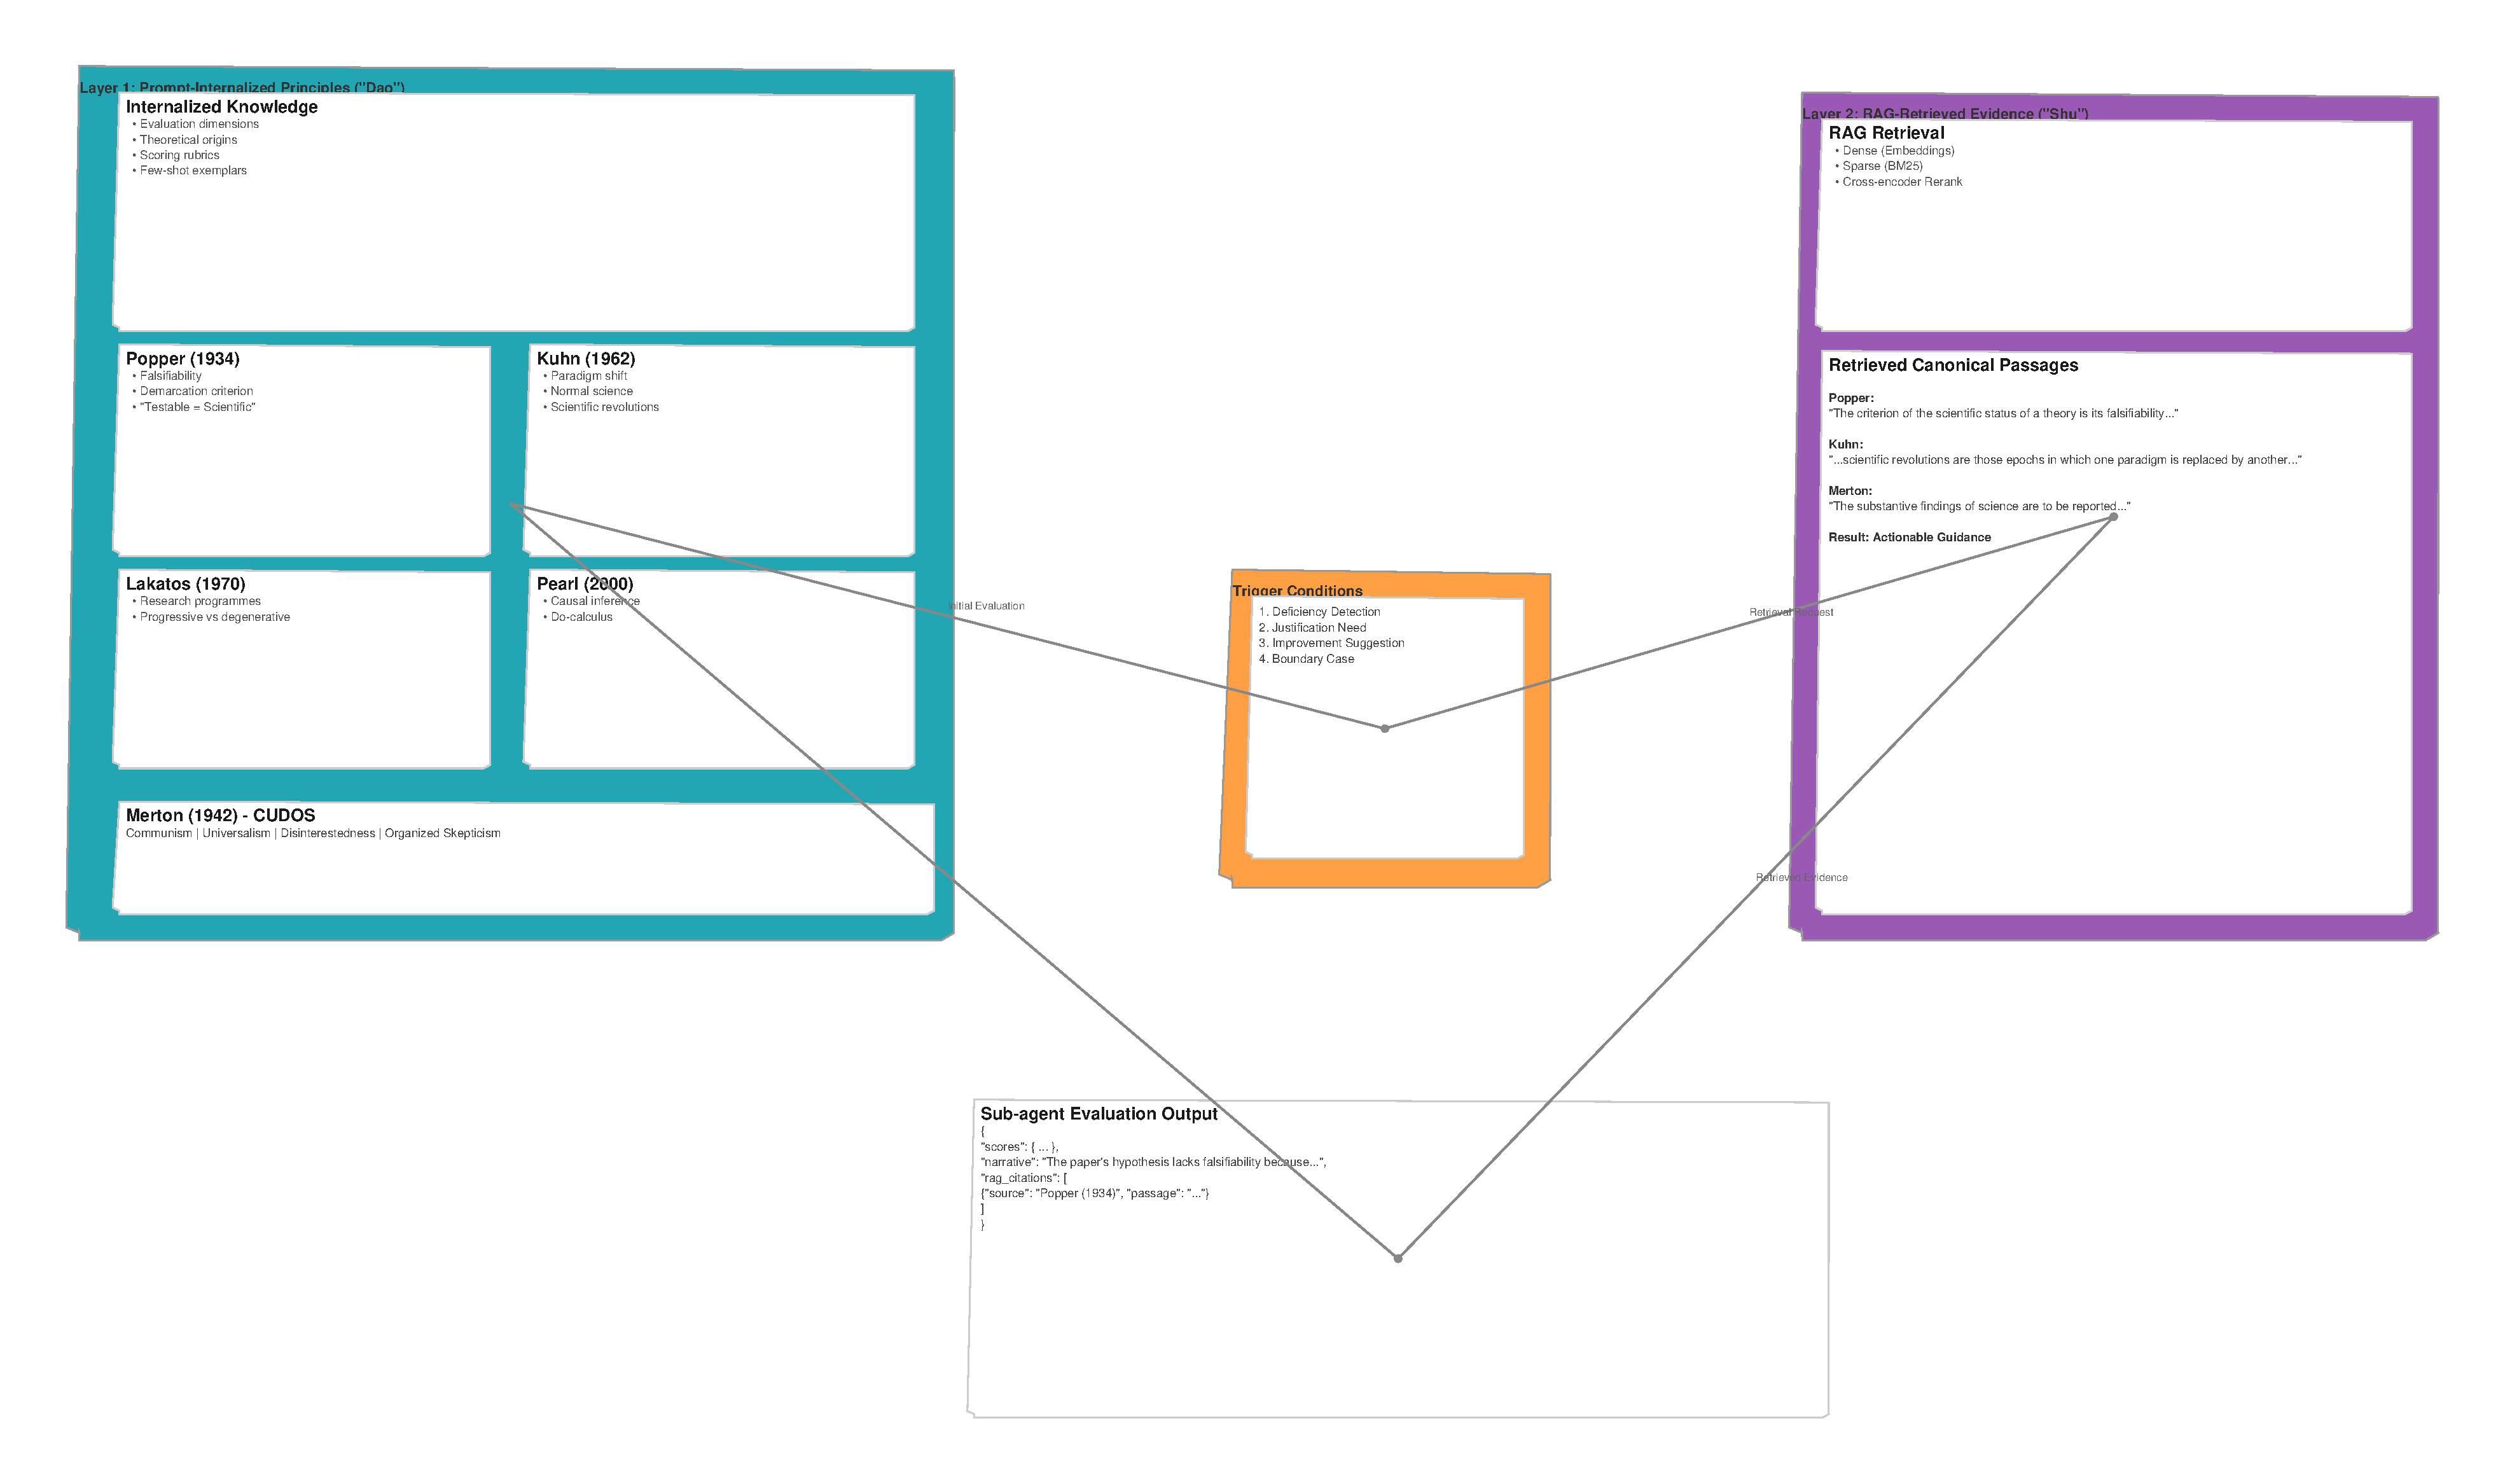
\includegraphics[width=0.8\textwidth]{figures/hybrid-knowledge.pdf}
    \caption{Hybrid Knowledge Strategy: Prompt-Internalized Principles + RAG-Retrieved Evidence}
    \label{fig:hybrid-knowledge}
\end{figure}

\textbf{Layer 1: Prompt-Internalized Principles (``Dao'').} Each \subagent{}'s system prompt contains:
\begin{itemize}
    \item The evaluation dimension and its theoretical origin.
    \item The multi-level structure: dimension $\rightarrow$ sub-dimensions $\rightarrow$ scoring criteria.
    \item Exemplars of evaluation at each score level.
    \item Boundary conditions and edge cases.
\end{itemize}

This internalized knowledge ensures consistent judgment without retrieval overhead.

\textbf{Layer 2: RAG-Retrieved Evidence (``Shu'').} When triggered, the RAG layer retrieves from a corpus of canonical texts indexed by:
\begin{itemize}
    \item \textbf{Theorist}: e.g., Popper, Kuhn, Campbell, Pearl.
    \item \textbf{Concept}: e.g., falsifiability, paradigm shift, internal validity.
    \item \textbf{Function}: explanation, critique, improvement suggestion.
\end{itemize}

The retrieved passages provide concrete justification that transforms abstract principles into actionable guidance. For example, when the Evidence Sub-agent identifies a falsifiability problem, it retrieves Popper's original text explaining what makes a hypothesis scientific, enabling it to provide specific suggestions for improvement.

\subsection{Sub-agent Specifications}

Each expert \subagent{} follows a consistent output schema while maintaining specialized evaluation logic:

\begin{verbatim}
{
  "dimension": "evidence_confidence",
  "scores": {
    "falsifiability": 3,
    "evidence_strength": 4,
    "replicability": 3,
    "research_program": 4
  },
  "narrative": "The paper's main hypothesis is testable...",
  "rag_citations": [
    {
      "source": "Popper (1934)",
      "passage": "The criterion of the scientific status...",
      "relevance": "Explains why falsifiability matters"
    }
  ]
}
\end{verbatim}

This standardized output enables consistent aggregation and comparison across dimensions.
